The simplest case in astrophysical fluid dynamics is that of \textbf{hydrostatic equilibrium}, where all of the fields are \textbf{static} and the system's forces are in \textbf{equilibrium}. In this scenario, the \textbf{continuity equation} is trivial, and the \textbf{Euler Equation} reduces to the form
\[
\frac{\nabla p}{\rho} = -\nabla \Phi.
\]
In this section, we'll go through a few classic examples of this.

\section{The Isothermal Slab}

One of the classic problems in hydrostatic equilibrium is the \textbf{isothermal slab}: an infinite, plane-parallel atmosphere in a uniform gravitational field. This toy model illustrates the key balance between pressure gradients and gravity in a simple geometry and has wide applications ranging from stellar atmospheres to thin galactic disks.

We consider a static system where the density profile \( \rho(z) \) depends only on the vertical coordinate \( z \), with symmetry about the midplane \( z = 0 \). The fluid is in hydrostatic equilibrium, and thus the Euler equation becomes:
\[
\frac{dP}{dz} = - \rho \frac{d\Phi}{dz}.
\]

Assuming the gas is \textbf{isothermal} with temperature \( T \), the pressure and density are related by:
\[
P = \frac{k_B T}{\mu m_p} \rho \equiv \alpha \rho,
\]
where \( \alpha \equiv \frac{k_B T}{\mu m_p} \) is a constant. Substituting this into the Euler equation gives:
\[
\alpha \frac{d\rho}{dz} = -\rho \frac{d\Phi}{dz} \quad \Rightarrow \quad \alpha \frac{d\log \rho}{dz} = -\frac{d\Phi}{dz}.
\]
Integrating, we obtain:
\[
\alpha \log \left( \frac{\rho(z)}{\rho_0} \right) = -\left[ \Phi(z) - \Phi_0 \right],
\]
or equivalently:
\[
\boxed{
\rho(z) = \rho_0 \exp\left[-\frac{\Phi(z) - \Phi_0}{\alpha}\right].
}
\]

To find \( \Phi(z) \), we now turn to the \textbf{Poisson equation} in one dimension:
\[
\frac{d^2 \Phi}{dz^2} = 4\pi G \rho(z).
\]
Substituting the expression for \( \rho(z) \) from above, we get:
\[
\frac{d^2 \Phi}{dz^2} = 4\pi G \rho_0 \exp\left[-\frac{\Phi(z) - \Phi_0}{\alpha}\right].
\]

Letting \( \psi(z) = \Phi(z) - \Phi_0 \), this becomes a nonlinear second-order ODE:
\[
\frac{d^2 \psi}{dz^2} = 4\pi G \rho_0 e^{-\psi/\alpha}.
\]

This equation has a well-known analytic solution. Solving and transforming back, we obtain the final result:

\begin{tcolorbox}[colback=blue!5!white,colframe=blue!75!black,title=Isothermal Slab Solution]
The gravitational potential and density profiles in an isothermal slab are given by:
\begin{equation}
    \label{eq:isothermal_slab}
\rho(z) = \rho_0 \, \mathrm{sech}^2 \left( \frac{z}{H} \right), \quad
\Phi(z) - \Phi_0 = 2\alpha \log \cosh\left(\frac{z}{H}\right),
\end{equation}
where the scale height is
\[
\boxed{
H = \sqrt{\frac{\alpha}{2\pi G \rho_0}}.
}
\]
\end{tcolorbox}

This solution describes a self-gravitating, plane-parallel atmosphere in thermal equilibrium, where pressure support exactly balances the slab’s self-gravity.

\subsection{Isothermal Slabs as Disks}

Astrophysical disks that are much thinner than their radius — such as \textbf{accretion disks} or \textbf{galactic disks} — are often well-described (in the vertical direction) by the isothermal slab approximation. The key requirements are:
\begin{itemize}
    \item The disk is \textbf{geometrically thin} ($H \ll R$),
    \item Vertical columns of gas cool efficiently and are approximately \textbf{isothermal},
    \item The pressure and density are related by a \textbf{barotropic equation of state} of the form \( P = \alpha \rho \), with constant \( \alpha \propto T \).
\end{itemize}

In many cases, the dominant gravitational potential is not sourced by the disk itself but by a \textbf{central body} (e.g., star, black hole) or external galactic potential. We must therefore consider a general potential \( \Phi(r,z) \), which varies in both the radial and vertical directions.

For a thin disk, we assume that most of the gravitational variation with height occurs close to the midplane. Thus, we expand the gravitational potential as a Taylor series in $z$:
\[
\Phi(r,z) = \Phi(r,0) + \left.\frac{\partial \Phi}{\partial z}\right|_{z=0} z + \frac{1}{2} \left.\frac{\partial^2 \Phi}{\partial z^2}\right|_{z=0} z^2 + \mathcal{O}(z^3).
\]
However, for disks symmetric about the midplane ($z = 0$), the odd derivatives vanish, so the linear term is absent:
\[
\Phi(r,z) = \Phi(r,0) + \frac{1}{2} z^2 \left.\frac{\partial^2 \Phi}{\partial z^2}\right|_{z=0} + \mathcal{O}(z^4).
\]
Now consider vertical hydrostatic equilibrium:
\[
\frac{dP}{dz} = -\rho \frac{d\Phi}{dz}.
\]
Using the isothermal assumption \( P = \alpha \rho \), we obtain:
\[
\alpha \frac{d\rho}{dz} = -\rho \frac{d\Phi}{dz}.
\]
Dividing both sides by \( \rho \) and integrating:
\[
\alpha \frac{d \log \rho}{dz} = -\frac{d\Phi}{dz} \implies \alpha \log \left( \frac{\rho}{\rho_0} \right) = -\left[ \Phi(r,z) - \Phi(r,0) \right].
\]
Substituting the second-order potential expansion:
\[
\alpha \log \left( \frac{\rho}{\rho_0} \right) = -\frac{1}{2} z^2 \left.\frac{\partial^2 \Phi}{\partial z^2} \right|_{z=0},
\]
which gives the vertical density profile:
\[
\boxed{
\rho(z) = \rho_0 \exp\left( - \frac{z^2}{2H^2} \right),
}
\quad \text{where} \quad H(r) = \sqrt{ \frac{\alpha}{ \left. \frac{\partial^2 \Phi}{\partial z^2} \right|_{z=0} } }.
\]

This is a \textbf{Gaussian density profile}, and $H(r)$ defines the local \textbf{scale height} of the disk. Since \( \alpha \propto T \), the scale height depends on both the local temperature and the curvature of the gravitational potential in the vertical direction.

\subsection{Other Uses of the Isothermal Slab Approximation}

The isothermal slab model is widely used in astrophysics to describe vertically stratified systems where thermal equilibrium and efficient cooling make the isothermal assumption valid. Below are several classic and practical use cases:

\begin{enumerate}
    \item \textbf{Stellar Atmospheres} \\
    In models of stellar atmospheres, particularly for stars with extended or radiative envelopes, the temperature gradient can be small over certain vertical layers. In these regimes, the atmosphere may be approximated as locally isothermal, simplifying analytic estimates of pressure and density stratification.

    \item \textbf{Molecular Cloud Cores and Sheets} \\
    In flattened molecular cloud cores or planar sheets within larger clouds, the vertical structure can be modeled as an isothermal slab during the early, quasi-static phases of evolution. Efficient cooling from dust and molecular lines keeps the temperature uniform, and the slab model aids in assessing gravitational stability.

    \item \textbf{Self-Gravitating Midplanes of Disks} \\
    When the disk’s own gravity becomes significant, the vertical profile may resemble a self-gravitating slab. This leads to solutions such as the classic Spitzer $\mathrm{sech}^2$ profile. Such models are used to explore fragmentation thresholds, disk midplane pressure, and star formation in dense disk environments.

    \item \textbf{Numerical Subgrid Models} \\
    In simulations where vertical resolution is limited (e.g., 2D simulations of disks), the vertical structure is often modeled as an isothermal slab. This assumption enables closure of the hydrodynamic equations without explicitly evolving the vertical temperature or density profile.

    \item \textbf{Photoionized Regions} \\
    In some HII regions or photoionized slabs, the temperature may be regulated by the balance of photoheating and line cooling. If this balance is efficient and uniform, the slab can be modeled as isothermal for purposes of calculating recombination rates, emission line profiles, and radiation transfer.
\end{enumerate}

\section{Stellar Polytropes}

Stellar polytropes are a classical model for the structure of a star which is not rotating and therefore maintains spherical symmetry. Because these are relatively easy to derive and interact with, they are ubiquitous in the literature, particularly in the context of dynamical modeling. In this section, we'll talk about the relevant physics and derive the core equations.
\par
In this scenario, we once again consider the Euler equation in the form
\[
\frac{\nabla P}{\rho} = -\nabla \Phi.
\]
There is rather a nice feature of these objects: They are \textbf{physically barotropic}. Note that $\Phi$ is a \textit{monotonically increasing function of radius}. As such, (because $\rho > 0$), $\nabla P < 0$, so $P$ must be \textit{monotonically decreasing with radius.} We therefore stumble onto a nice property:
\begin{center}
    The \textbf{level surfaces} of $\Phi$, $P$, and $\rho$ coincide. Furthermore, because $P$ and $\Phi$ are monotonic, we can write $P(\Phi)$ and $\rho(\Phi)$.
\end{center}
\par
From this statement, we can immediately recognize that
\[
\rho = - \frac{\partial P}{\partial \Phi},
\]
and that we we have a \textbf{barotropic equation of state}: $P(\rho)$. Here's the problem, we don't actually know what $P(\rho)$ is going to be... We will therefore choose a \textbf{parameterization}.
\vspace{0.5cm}
\begin{proposition}
    Consider the scenario where $P(\rho)$ is a \textbf{polytrope} of the form
    \[
    P = K \rho^{1+1/n}
    \]
    for some \textbf{polytropic index $n$.}
\end{proposition}
\vspace{0.5cm}
As we will see, this leads us directly to the famous \textbf{Lane-Emden equation}, which is used in many scenarios to study the structures of stars.

\subsection{The Lane-Emden Equation}

We may begin by substituting the equation of state into the \textbf{Euler Equation} (equation~\ref{eq:conservation-equation-lagrangian}) to obtain
\[
- \nabla \Phi = \frac{K}{\rho} \nabla \rho^{1+1/n} = (n+1)K \nabla \rho^{1/n}.
\]
\rmk{This manipulation to put $\rho$ back on the inside is a little tricky and worth reviewing.} Integrating this equation between some $(\Phi_0,\rho_0)$ and some $(\Phi_1,\rho_1)$, we find
\begin{equation}
    \Phi_1 - \Phi_0 = (n+1)K \left(\rho_{0}^{1/n} - \rho_1^{1/n}\right)
\end{equation}
We will find it convenient to introduce the points $(\Phi_C,\rho_C)$ corresponding to the \textbf{center of the star} and 
$(\Phi_T,0)$, corresponding to the \textbf{edge (truncation radius)} of the star. This allows us to express $\rho(\Phi)$ as 
\[
\rho(\Phi) = \left(\frac{\Phi_T-\Phi}{(n+1)K}\right)^n.
\]
\par
We have effectively \textbf{eliminated the pressure}, we now wish to \textbf{eliminate $\Phi$} to obtain a single ODE which can be integrated. To do so, we use the \textbf{Poisson Equation}:
\[
\nabla^2 \Phi = \frac{1}{r^2} \partial_r \left(r^2\partial_r \Phi\right) = 4\pi G \rho = 4\pi G\underbrace{\left(\frac{\Phi_0-\Phi}{(n+1)K}\right)^n}_{\rho}
\]
This is now a \textbf{single-variable ODE} which we could naively integrate the solve our problem; however, it is worthwhile to attempt to remove any dimensional dependence from the problem. This is of particular use when studying the mathematics of solutions.
\par
To eliminate the units of the \textbf{potential}, we can introduce the scale-free potential
\[
\Theta(r) = \frac{\Phi_T-\Phi}{\Phi_T-\Phi_C}.
\]
\rmk{The idea here is that $\Theta$ goes from $0$ at the \textbf{truncation point} to $1$ at the center and doesn't have any units.} In these units, the density also becomes
\begin{equation}
\label{eq:LE-density}
\boxed{
\rho = \rho_C \Theta^n,\;\rho_C = \left(\frac{\Phi_T-\Phi_C}{(n+1)K}\right)^n
}
\end{equation}
where $\rho_C$ is the \textbf{central density}, which is general a free parameter of a given model.
\par
We'd also like to get rid of the length scale of the problem: $r$. To do so, we need to define a scale radius $\alpha$, which is conveniently
\begin{equation}
    \label{eq:LE-length}
    \boxed{
    \xi = \left(\frac{4\pi G \rho_C}{\Phi_T-\Phi_C}\right)^{1/2} r = \alpha r.
    }
\end{equation}
In these units, the \textbf{Lane-Emden Equation} finally reveals itself:
\begin{equation}
    \label{eq:Lane-Emden}
    \boxed{
    \frac{1}{\xi^2} \partial_\xi \left(\xi^2 \partial_\xi \Theta\right) = - \Theta^n.
    }
\end{equation}
\begin{remark}
    It is worth recognizing that, at this stage, knowledge of $\Theta(\xi)$ can then be inverted to find $\rho$, and to find $r$, and then to reconstruct $\Phi(r)$, etc. The benefit is that all of the physical scaling is gone from the Lane-Emden equation, now its just math.
\end{remark}
\begin{figure}[ht!]
    \centering
    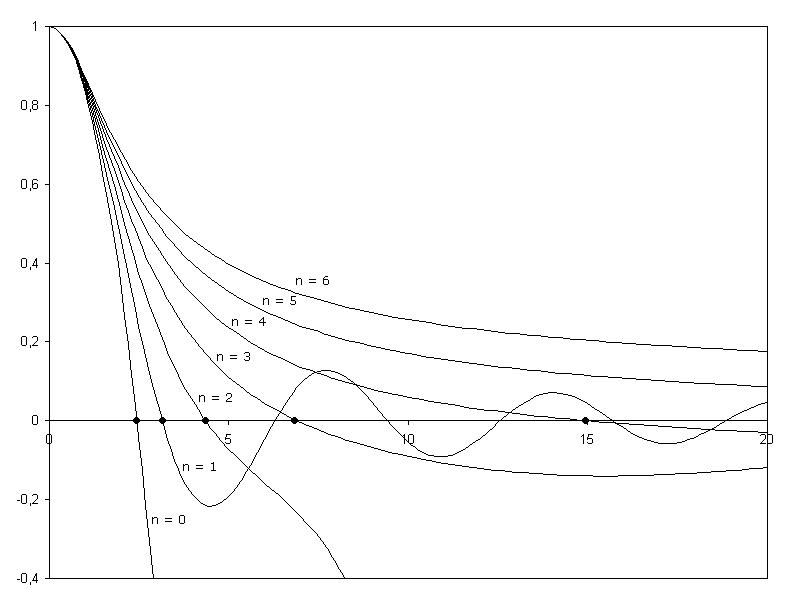
\includegraphics[width=0.75\linewidth]{Pictures/figures/Lane-emden.jpeg}
    \caption{Solutions to the Lane-Emden equation subject to the boundary conditions discussed in this section. Note the appearance of zeros in the solutions, which are representative of the truncation radius.}
    \label{fig:lane-emden}
\end{figure}
\subsection{General Properties of the Lane-Emden Equation}

It is worthwhile to study some of the very basic details of the Lane-Emden equation (equation~\ref{eq:Lane-Emden}) in order to get a feel for the sorts of solutions that arise from this problem. In general, one \textbf{needs to numerically integrate} the Lane-Emden (LE) equation in order to find solutions; however, special exceptions to this behavior exist for \framebox{$n = 0, 1, 5$.} We will study these solutions below in more detail.
\par
Before discussing solutions, we first need to discuss the \textbf{boundary conditions} for the LE equation. We are interested in solutions of the LE equation on domains characterized by the a specific \textbf{truncation radius (surface radius)} $r_T$: $D = [0,r_T] \subset \mathbb{R}$. Corresponding to this, we have $\xi \in [0,\xi_T]$; however, we \textbf{don't actually know $\xi_T$.} Instead, we recognize that, at $\xi = \xi_T$, we require that $\Theta = 0$ corresponding to \textbf{zero-density}. Thus, \framebox{$\xi_T$ is the \textbf{first zero} of the solution.}
\par
At $\xi = 0$, we need 
\[
\rho = \rho_C \Theta^n = \rho_C \implies \Theta(\xi = 0) = 1.
\]
Likewise, because $\Theta$ is a \textbf{scale-free potential}, 
\[
\frac{d\Theta}{d\xi} \propto \frac{d\Phi}{dr} = 0\;\text{by Gauss' Law.}
\]
Thus, we are interested in solving the following \textbf{Boundary Value Problem (BVP):}
\begin{equation}
\boxed{
    \frac{1}{\xi^2}\partial_\xi\left(\xi^2 \partial_\xi \Theta\right)  - \Theta^n = 0\;\; \text{where}\;\;\xi \in [0, \xi_T],\; \Theta(0) = 1,\; \Theta'(0) = 0.}
\end{equation}

We will now discuss specific solutions which are analytically known.

\subsubsection{The $n=0$ Solution}

For $n=0$, the LE equation takes the form
\begin{equation}
    \partial_\xi \left(\xi^2 \partial_\xi \Theta\right) = - \xi^2,
\end{equation}
which can be integrated once in the form
\[
\int \frac{\partial}{\partial \xi}\left(\xi^2 \frac{\partial \Theta}{\partial \xi}\right) \;d\xi = \xi^2 \frac{\partial \Theta}{\partial \xi} = - \frac{1}{3}\xi^3 + C_0.
\]
Integrating again yields
\[
\frac{\partial \Theta}{\partial \xi} =-\frac{1}{3} \xi + C_0\xi^{-2} \implies \Theta = -\frac{1}{6}\xi^2 - \frac{C_0}{\xi} + C_1.
\]
In order to \textbf{avoid asymptotic behavior} as $\xi \to 0$, we need $C_0 = 0$. Likewise, at $\xi = 0$, we need $C_1 = 1$ to match our boundary conditions. Therefore,
the solution is
\begin{equation}
\label{eq:solution_n1_le}
    \boxed{
    \Theta(\xi) = 1 - \frac{1}{6}\xi^2.
    }
\end{equation}
\par
The boundary occurs at the first $\Theta = 0$, which occurs at $\xi_T = \sqrt{6}$. 

\subsubsection{The $n=1$ Solution}

For the $n=1$ case, we have 
\[
\frac{1}{\xi^2} \frac{\partial }{\partial \xi}\left(\xi^2 \frac{\partial \Theta}{\partial \xi}\right) = \frac{\partial^2 \Theta}{\partial \xi^2} + \frac{2}{\xi} \frac{\partial \Theta}{\partial \xi} + \Theta = 0.
\]
We solve this by \textbf{power-law methods}: consider a solution
\[
\Theta(\xi) = \sum_{n=0}^\infty \alpha_n \xi^n,
\]
then
\[
\sum_{n=0}^\infty (n+2)(n+1) \alpha_{n+2} \xi^{n} \;+ \sum_{n=0}^\infty 2(n+2) \alpha_{n+2} \xi^n + \sum_{n=0}^\infty \alpha_n \xi^n = 0.
\]
Equating terms, we find
\[
(n+2)(n+3) \alpha_{n+2} + \alpha_n = 0 \implies \alpha_{n+2} = \frac{\alpha_n}{(n+2)(n+3)}.
\]
If we start from some $\alpha_0$, then
\[
\alpha_{2k} = \frac{(-1)^k}{(2k +1)!}\alpha_0.
\]
We could do the same for the odd elements, but we recognize that $\alpha_1 = 0$ by our boundary conditions. A quick look at a Taylor-Series table shows that this power law corresponds to 
\[
\Theta(\xi) \sim \alpha_0 \frac{\sin \xi}{\xi}.
\]
To maintain the boundary condition, we have
\begin{equation}
    \Theta(\xi) = \frac{\sin \xi}{\xi}.
\end{equation}
Clearly, in this case, \framebox{$\xi_T = \pi$.}
\begin{remark}
    This is actually even easier with the substitution $\chi = \Theta \xi$, in which case the equation takes the form
    \[
    \frac{d^2\chi}{d\xi^2} = - \chi^n/\xi^{n-1}.
    \]
    which is a simple second order ODE.
\end{remark}

\subsubsection{The $n=5$ Solution}

We start from the Lane Emden equation:
\begin{equation}
    \frac{1}{\xi^{2}} \frac{d}{d\xi} \left(\xi^{2} \frac{d\theta}{d\xi}\right) + \theta^{5} = 0.
\end{equation}

Rewriting for the derivative $\tfrac{d\theta}{d\xi}$ produces
\begin{equation}
    \frac{d\theta}{d\xi} 
    = \frac{1}{2}\left(1+\frac{\xi^{2}}{3}\right)^{3/2} \cdot \frac{2\xi}{3}
    = \frac{\xi}{3}\left(1+\frac{\xi^{2}}{3}\right)^{-3/2}.
\end{equation}

Differentiating again with respect to $\xi$ leads to
\begin{equation}
    \theta^{5}
    = \frac{\xi^{2}}{\left(1+\frac{\xi^{2}}{3}\right)^{3/2}}
    + \frac{3\xi^{2}}{9\left(1+\frac{\xi^{2}}{3}\right)^{5/2}}
    = \frac{9}{9\left(1+\frac{\xi^{2}}{3}\right)^{5/2}}.
\end{equation}

This reduces to
\begin{equation}
    \theta^{5} = \frac{1}{\left(1+\frac{\xi^{2}}{3}\right)^{5/2}}.
\end{equation}

Therefore, the Lane--Emden equation has the analytic solution
\begin{equation}
    \theta(\xi) = \frac{1}{\sqrt{1+\xi^{2}/3}}, \qquad n=5.
\end{equation}

This solution corresponds to a configuration of finite mass but infinite radial extent. 

\subsection{Scaling Relations of the Lane-Emden Equation}

We \textbf{cannot generally solve} the Lane-Emden equation; however, we can derive various scaling relationships between the relevant quantities in the equations. This is useful as it can tell us (\textbf{for fixed $n$}) how certain properties scale with one another. The core of this idea is that \textit{regardless of scaling}, $\Theta_n(\xi)$ is a \textbf{fixed function for each index}. As such, different physical solutions for the same $n$ are forced to have similar properties.
\par
Assume that we have, by numerical integration or otherwise, obtained a solution $\Theta(\xi)$ for a particular index $n$. we know that $\xi$ and $\Theta$ are defined (see equation~\ref{eq:LE-length} and \eqref{eq:LE-density}) such that
\[
    \xi = \left(\frac{4\pi G \rho_C}{\Phi_T-\Phi_C}\right)^{1/2} r = \alpha r,
\]
and
\[
\rho = \rho_C \Theta^n,\;\rho_C = \left(\frac{\Phi_T-\Phi_C}{(n+1)K}\right)^n.
\]
Substituting the expression for $\rho_C$ into $\alpha$, we find that
\begin{equation}
    \boxed{
    \xi = \left(\frac{4\pi G \rho_C^{1-(1/n)}}{K(n+1)}\right)^{1/2}r,
    }
\end{equation}
which gives us an exact scaling on the \textbf{maximum radius} in terms of the \textbf{core density}:
\begin{equation}
    \label{eq:LE-scaling-radius}
    R_{\rm max} = \alpha \xi_{T} \propto \rho_C^{(n-1)/2n}.
\end{equation}
\par
We may also then ask about the scaling of the total mass with the core density and the radius. Clearly, if 
\[
\rho \sim \rho_C \Theta^n, \implies M = 4\pi \rho_C \alpha^{-3} \int_0^{\xi_T}\;d\xi \;\Theta^n \xi^2 \propto \rho_C \alpha^{-3}. 
\]
Since $\alpha \sim \rho_C^{(n-1)/2n}$, we know that
\[
M \sim \rho_C \rho_C^{-3(n-1)/2n} = \rho_c^{(3-n)/2n}
\]
Comparing this to the scaling for $R$, we have
\[
M \sim R^{(3-n)/(1-n)}.
\]

\subsection{Bonnor-Ebert Spheres}

When \( n = \infty \), we obtain the \textbf{isothermal equation of state}, 
\[
P = K \rho,
\]
which implies
\[
K \nabla \log \rho = \nabla \Phi \quad \Rightarrow \quad \rho = \rho_0 \exp\left(-\frac{\Phi - \Phi_0}{K}\right).
\]
Substituting this relation into the Poisson equation,
\[
\nabla^2 \Phi = 4\pi G \rho,
\]
we obtain:
\[
\nabla^2 \Phi = 4\pi G \rho_0 \exp\left(-\frac{\Phi - \Phi_0}{K}\right).
\]
Now, define a dimensionless potential:
\[
\psi \equiv \frac{\Phi - \Phi_0}{K}, \quad \text{so that} \quad \rho = \rho_0 e^{-\psi}.
\]
Then the equation becomes:
\[
\nabla^2 \psi = \frac{4\pi G \rho_0}{K} e^{-\psi}.
\]

To nondimensionalize, define a radial coordinate:
\[
\xi \equiv \frac{r}{r_0}, \quad \text{with} \quad r_0^2 = \frac{K}{4\pi G \rho_0}.
\]
Then the Laplacian in spherical symmetry becomes:
\[
\frac{1}{r^2} \frac{d}{dr} \left( r^2 \frac{d\psi}{dr} \right)
= \frac{1}{r_0^2 \xi^2} \frac{d}{d\xi} \left( \xi^2 \frac{d\psi}{d\xi} \right).
\]
Thus, the final form of the \textbf{isothermal Lane–Emden equation} is:
\[
\boxed{
\frac{1}{\xi^2} \frac{d}{d\xi} \left( \xi^2 \frac{d\psi}{d\xi} \right) = e^{-\psi}.
}
\]
This is the equation that governs the structure of the \textbf{isothermal sphere}. 

\subsubsection{Bonnor-Ebert Spheres}

Assume a power-law behavior for the density at large \( \xi \),
\[
\rho(\xi) \propto \xi^{-n} \quad \Rightarrow \quad \psi(\xi) = n \log \xi + \text{const}.
\]

Then compute derivatives:
\[
\frac{d\psi}{d\xi} = \frac{n}{\xi}, \qquad \frac{d^2\psi}{d\xi^2} = -\frac{n}{\xi^2}.
\]

Substitute into the left-hand side of the equation:
\[
\frac{d^2\psi}{d\xi^2} + \frac{2}{\xi} \frac{d\psi}{d\xi} = -\frac{n}{\xi^2} + \frac{2n}{\xi^2} = \frac{n}{\xi^2}.
\]

On the right-hand side:
\[
e^{-\psi} = e^{-n \log \xi + \text{const}} = C \cdot \xi^{-n}.
\]
To be consistent, both sides must scale the same way, so:
\[
\frac{n}{\xi^2} \propto \xi^{-n} \quad \Rightarrow \quad n = 2.
\]

\begin{tcolorbox}[colback=blue!5!white, colframe=blue!75!black, title=Asymptotic Form]
At large radii, the solution to the isothermal Lane-Emden equation behaves as:
\[
\boxed{
\rho(\xi) \propto \xi^{-2}, \qquad \psi(\xi) \sim 2 \log \xi + \text{const}.
}
\]
This is the familiar result for the singular isothermal sphere.
\end{tcolorbox}

Here's the problem: \textbf{this means the mass is infinite}. So what happens if we instead force the system to truncate at a particular radius $r_t$? In that case, we need to introduce an \textbf{external pressure source} in order to make up for the missing gravitational mass. Since $P = K \rho$, we can simply say that
\[
P_{\rm ext} = K \rho(r_T).
\]
\subsubsection{Stability of Bonnor–Ebert Spheres}

A natural question is: \textbf{what happens when we perturb the truncation radius $r_T$ slightly}? For instance, a small compression of the sphere might result from infalling material, a shock, or some internal perturbation. The key diagnostic is the response of the required external pressure $P_{\rm ext}$. If $P_{\rm ext}$ increases to oppose the compression, the configuration is stable; if $P_{\rm ext}$ decreases, the configuration is unstable and the collapse may run away.

We consider a family of truncated isothermal spheres with central density $\rho_c$, truncated at radius $r_T$, and held in equilibrium by an external pressure $P_{\rm ext}$. From the isothermal Lane–Emden solution, we define:

\begin{itemize}
    \item The dimensionless radius: $\xi = r / R_0$, where $R_0^2 = \alpha / (4\pi G \rho_c)$,
    \item The dimensionless potential: $\psi(\xi)$ such that $\rho(\xi) = \rho_c e^{-\psi(\xi)}$,
    \item The \textbf{mass function} (not the actual mass!):
    \[
    m(\xi) = \xi^2 \frac{d\psi}{d\xi}.
    \]
\end{itemize}

Then, the pressure at the outer boundary is
\[
P_{\rm ext} = K\rho(\xi_T) = K\rho_c e^{-\psi(\xi_T)}.
\]

We now vary $\xi_T$ slightly and track the behavior of $P_{\rm ext}$. Taking the derivative:
\[
\frac{dP_{\rm ext}}{d\xi_T} = - K \rho_c e^{-\psi(\xi_T)} \frac{d\psi}{d\xi_T}.
\]
This shows that the sign of $dP_{\rm ext}/d\xi_T$ \textbf{depends entirely on the slope $d\psi/d\xi_T$ at the boundary.}

From the Lane–Emden equation:
\[
\frac{1}{\xi^2} \frac{d}{d\xi}\left( \xi^2 \frac{d\psi}{d\xi} \right) = e^{-\psi},
\]
we can numerically solve for $\psi(\xi)$ and its derivatives. One then computes $dP_{\rm ext}/d\xi_T$ and finds that:

\begin{itemize}
    \item For $\xi_T < \xi_{\rm crit} \approx 6.451$, the derivative is negative: compressing the sphere increases $P_{\rm ext}$, which resists the compression. This implies \textbf{stability}.
    \item For $\xi_T > \xi_{\rm crit}$, the derivative is positive: compressing the sphere decreases $P_{\rm ext}$, which fails to resist collapse. This implies \textbf{instability}.
\end{itemize}

Thus, the function $P_{\rm ext}(\xi_T)$ reaches a minimum at $\xi_T = \xi_{\rm crit}$. Beyond this point, the configuration cannot remain in equilibrium without fine-tuned external support. Thus, the Bonnor–Ebert sphere provides a natural \textbf{threshold model for gravitational collapse}.

\begin{tcolorbox}[colback=red!5!white, colframe=red!75!black, title=Bonnor–Ebert Stability Criterion]
A Bonnor–Ebert sphere is:
\begin{itemize}
    \item \textbf{Stable} if $\xi_T < \xi_{\rm crit} \approx 6.451$,
    \item \textbf{Unstable} if $\xi_T > \xi_{\rm crit}$.
\end{itemize}
The instability corresponds to collapse under self-gravity once external pressure support becomes insufficient.
\end{tcolorbox}

\subsection{Implications of Polytropic Models and Bonnor–Ebert Spheres}

Polytropic models provide a powerful, unifying framework for understanding the structure of self-gravitating astrophysical objects under hydrostatic equilibrium. The simplicity of the polytropic equation of state,
\[
P = K \rho^{1 + 1/n},
\]
permits analytic and semi-analytic solutions to otherwise intractable stellar structure problems. Their implications span a wide range of astrophysical scenarios:

\begin{enumerate}
    \item \textbf{Unified Treatment of Stellar Interiors} \\
    Many types of stars — from low-mass dwarfs to massive stars — are approximately modeled by different polytropic indices. For example:
    \begin{itemize}
        \item Fully convective stars $\rightarrow$ $n \approx 1.5$,
        \item Degenerate cores or white dwarfs $\rightarrow$ $n \approx 1.5$ (non-relativistic) or $n = 3$ (ultrarelativistic),
        \item Radiation-pressure dominated massive stars $\rightarrow$ $n \rightarrow 3$.
    \end{itemize}
    This enables comparison across different evolutionary stages and mass regimes.

    \item \textbf{Insights into Stellar Stability and Limits} \\
    The solutions to the Lane–Emden equation for various $n$ reveal key stability properties. For instance, polytropes with $n < 5$ have finite radius and mass, while those with $n \geq 5$ are unbounded. This connects directly to phenomena like the Chandrasekhar mass limit and the onset of instability in massive stars.

    \item \textbf{Analytic Scaling Relations} \\
    Polytropes yield closed-form scaling laws for core pressure, density, temperature, and radius as functions of mass and composition. These relations are essential for interpreting observations and for initializing stellar evolution models.

    \item \textbf{Bonnor–Ebert Spheres as Collapse Thresholds} \\
    The isothermal limit ($n = \infty$) leads to the Bonnor–Ebert sphere: a pressure-confined, self-gravitating equilibrium solution. This model provides a physically motivated criterion for gravitational instability in interstellar gas:
    \begin{itemize}
        \item For $\xi_T < \xi_{\rm crit} \approx 6.451$, the configuration is stable.
        \item For $\xi_T > \xi_{\rm crit}$, small perturbations lead to runaway collapse.
    \end{itemize}
    Observed molecular cloud cores that match the radial density profiles of Bonnor–Ebert spheres can be diagnosed as collapsing or stable depending on their dimensionless radius.

    \item \textbf{Connection to Star Formation} \\
    Bonnor–Ebert spheres offer one of the few analytic, observationally testable models for the initial stages of star formation. They predict the critical conditions — mass, temperature, external pressure — under which a prestellar core transitions from quasi-static equilibrium to gravitational collapse.

    \item \textbf{Bridge Between Microphysics and Macrophysics} \\
    Polytropic models illustrate how microphysical assumptions (e.g., ideal gas law, radiation pressure, degeneracy) manifest as macroscopic structure. The mapping from $n$ to physical processes connects thermodynamics, radiative transport, and hydrodynamics in a compact formalism.

\end{enumerate}

\section{The Intracluster Medium}

Galaxy clusters are composed of several mass components, approximately partitioned as:
\begin{itemize}
    \item \textbf{Dark Matter} — $\sim 85\%$
    \item \textbf{Hot Ionized Gas (Intracluster Medium)} — $\sim 14\%$
    \item \textbf{Stars in Galaxies} — $\sim 1\%$
\end{itemize}

The \textbf{intracluster medium (ICM)} is a hot ($T \sim 10^7$–$10^8$ K), diffuse plasma that emits strongly in the X-ray band via thermal bremsstrahlung and line emission. The X-ray surface brightness and spectral information allow observers to reconstruct the projected temperature and density profiles of the gas.

\subsection{Hydrostatic Equilibrium in the ICM}

For a galaxy cluster in approximate \textbf{hydrostatic equilibrium}, the pressure gradient in the ICM must balance the gravitational force from the total mass:
\[
\frac{dP}{dr} = -\rho_g(r) \frac{d\Phi}{dr},
\]
where:
\begin{itemize}
    \item $P(r)$ is the gas pressure,
    \item $\rho_g(r)$ is the gas density,
    \item $\Phi(r)$ is the total gravitational potential sourced by all mass components: dark matter, stars, and gas.
\end{itemize}

The pressure of the gas is related to its density and temperature by the ideal gas law:
\[
P(r) = \frac{k_B}{\mu m_p} \rho_g(r) T(r) \equiv K \rho_g(r) T(r),
\]
where:
\begin{itemize}
    \item $k_B$ is Boltzmann’s constant,
    \item $m_p$ is the proton mass,
    \item $\mu$ is the mean molecular weight (typically $\mu \approx 0.6$),
    \item $T(r)$ is the radial temperature profile.
\end{itemize}

\subsection{General Expression for the Dynamical Mass}

Applying the product rule and dividing by $\rho_g$, the hydrostatic balance becomes:
\[
\frac{1}{\rho_g} \frac{dP}{dr} = K \frac{dT}{dr} + K T \frac{d\log \rho_g}{dr} = -\frac{d\Phi}{dr}.
\]
The gravitational acceleration is related to the total enclosed mass $M_{\rm dyn}(<r)$ via:
\[
\frac{d\Phi}{dr} = \frac{G M_{\rm dyn}(<r)}{r^2}.
\]
Combining these gives:
\[
K \left( \frac{dT}{dr} + T \frac{d\log \rho_g}{dr} \right) = -\frac{G M_{\rm dyn}(<r)}{r^2}.
\]
Dividing both sides by $K$ and rearranging, we find the key relation for the enclosed dynamical mass:
\begin{tcolorbox}[colback=blue!5!white, colframe=blue!75!black, title=Hydrostatic Mass Equation for the ICM]
\begin{equation}
\boxed{
M_{\rm dyn}(<r) = -\frac{r^2}{G} \frac{k_B T(r)}{\mu m_p} \left[ \frac{d\log T}{dr} + \frac{d\log \rho_g}{dr} \right].
}
\end{equation}
\end{tcolorbox}

This expression allows observers to estimate the total (mostly dark) mass of a cluster using observed profiles of $T(r)$ and $\rho_g(r)$ under the assumption of hydrostatic equilibrium. It is widely used in X-ray and SZ studies of galaxy clusters.

\subsection{Limitations and Caveats}

\begin{itemize}
    \item The ICM is \textbf{not truly isothermal}; real temperature profiles typically decline at large radii.
    \item Non-thermal pressure support (e.g., turbulence, magnetic fields, cosmic rays) can cause hydrostatic mass estimates to \textbf{underestimate} the true mass.
    \item This method assumes \textbf{spherical symmetry} and \textbf{equilibrium}, which may be violated in merging or dynamically active clusters.
\end{itemize}

